\documentclass[12pt]{article}	

\usepackage[margin=1in]{geometry}
\usepackage{amsmath,amssymb,amsthm}
\usepackage{graphicx}
\usepackage{url}
\usepackage{mathrsfs}
\newtheorem{theorem}{Theorem}
\newtheorem{notation}{Notation}
\newtheorem{claim}{Claim}
\newtheorem{lemma}{Lemma}
\newtheorem{definition}{Definition}
\renewcommand{\qedsymbol}{$\blacksquare$}
\newtheorem*{remark}{Remark}

\begin{document}
	
	\begin{center}
		Homework 1
	\end{center} 
	{\rule{\linewidth}{0.1mm} }
	
	2. The taylor series approximation of $cos(x) = \sum\limits_{i=0}^{\infty} (-1)^n \frac{x^{2n}}{(2n)!}$. \\
	\indent The following is an image of the taylor series approximation up to second, fourth and twentieth order plotted against the original graph of $cos(x)$\\\\
	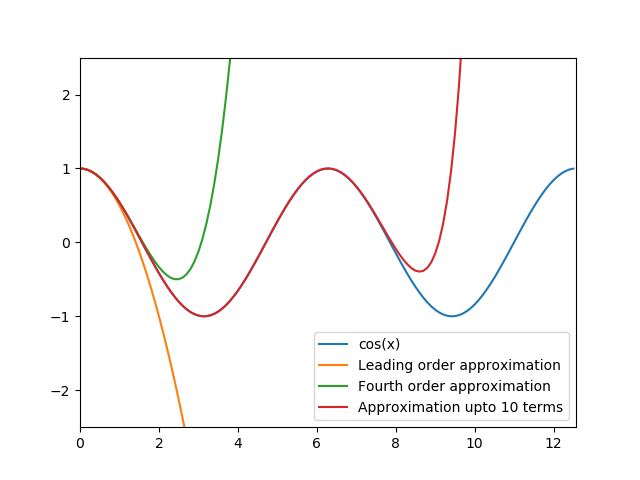
\includegraphics[scale=0.60]{2.png}\\
	\indent These approximations continue to approximate $cos(x)$ to a better and better degree with higher and higher orders. In order to understand this, we can study $|p_n(x)-cos(x)|$ where $p_n(x)$ is the $nth$ order approximation of $cos(x)$. Asymptotically, as $n \rightarrow \infty$ we expect our approximations to approach $g(x) = 0$. The following is the plot of $|p_2-cos(x)|, |p_4-cos(x)|$ and $|p_{20}-cos(x)|$, and it is evident that $p_n(x)$ is a better approximation as $n \uparrow$.
	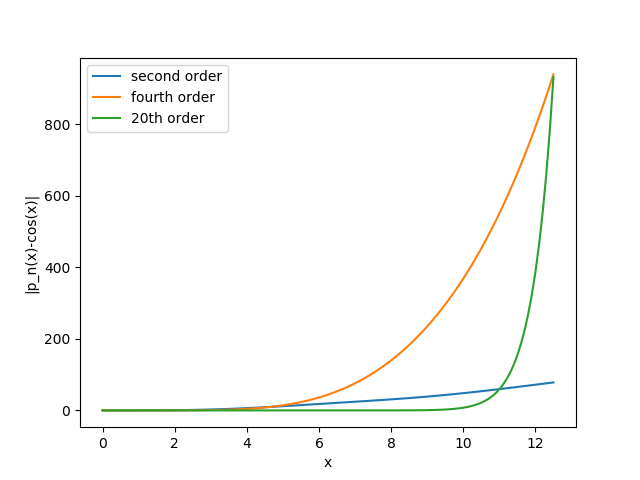
\includegraphics[scale=0.60]{2_deviation.png}\\
	
	\newpage
	
	3. The classical formula for variance is $E[x^2] - {E[x]}^2 = \frac{\sum_{i=1}^{N}(x_i - \bar{x})^2}{N-1} = \frac{\sum_{i=1}^{N}(x_i^2 - N\bar{x}^2)}{N-1} $. This is the formula that is computed in the first pseudocode. \\\\
	The second pseudocode, we use a technique attributed to Welford. Where, we consider the following "trick". Let $v_n$ be the variance of the first $n$ terms. Then it can be shown that \\
	\begin{center}$(N-1)v_N - (N-2)v_{N-1} = (x_N - \bar{x}_N)(x_N - \bar{x}_{N-1})$ \end{center}. \\ Welford's technique uses this method to recursively compute \\ $(N-1)v_N = (N-2)v_{N-1} + (x_N - \bar{x}_N)(x_N - \bar{x}_{N-1})$, and the end of the computation, we divide by $(N-1)$ to obtain $v_N$ as desired. \\ At each step, $\bar{x}_i$ is computed from $\bar{x}_{i-1}$ using the formula, $\bar{x}_i = \bar{x}_{i-1} + \frac{x_i-\bar{x}_{i-1}}{i}$
	\\\\
	In the third pseudocode, we use a technique similar to Welford, which is attributed to Youngs and Cramer. Their technique is similar to that of Welford's technique - and this can be attained by just a few algebraic manipulation of the mean terms that appear in Welford's formula. \\
		{\rule{\linewidth}{0.1mm} }\\
	 
	 4. A shooting method was implimented in python to solve the following boundary value problem
	$$y'' = -\pi^2 y$$ with the boundary constraints $y(0) = 0$ and $y(\frac{1}{2}) = 1$.
\\\\
Analytically, we can easily deduce (using the characteristic polynomial of this DE, or simply by observation) that the solution is $y=sin(\pi x)$. 
However, in order to solve this boundary value problem numerically, we turn the BV problem into a Initial value problem by assuming an arbitrary value $a$ for $y'(0)$. Let $z = y'(x)$
Now, we are equipped with the following Initial value problems in $z$, namely 
\begin{center}
	$z = y'(x) = f_1(x,y,z)$, \quad \quad $z(0) = a$ \\
	$z' = -\pi^2*y(x) = f_2(x,y,z)$, \quad \quad $y(0) = 0$ 
\end{center}		

Initially, we have $x=0, y=0, z=a$, therefore, we can numerically solve for the next data point (taking a stepsize $h$) for $x,y$ and $z$ using the discrete equations 
\begin{center}
	$x_{n} = x_{n-1} + h$\\
	$y_{n} = y_{n-1} + f_1(x_{n-1}, y_{n-1}, z_{n-1})h$\\
	$z_{n} = z_{n-1} + f_2(x_{n-1}, y_{n-1}, z_{n-1})h$
\end{center}

After iterating until $x=\frac{1}{2}$, we can check the value of $y(1/2)$ against $sin(\frac{\pi}{2}) = 1$. \\\\ 
We can now, iterate through other values of $a$, and plot $y(\frac{1}{2})$ against its respective $a$-value. The $a$ value at which this plot interescts the function $f(a) = 1 = sin(\frac{\pi}{2})$, will be the critical $a_0$ value for which our BVP is equal to the IVP with the IC being $y(0)=0, \ y'(0) = a_0$.   \\ \newpage
The plot of $y(\frac{1}{2})$ vs. $a$ is presented below. It is evident that it intersects the function $f(a) = 1$ at $\pi$ which we can analytically confirm is correct.\\
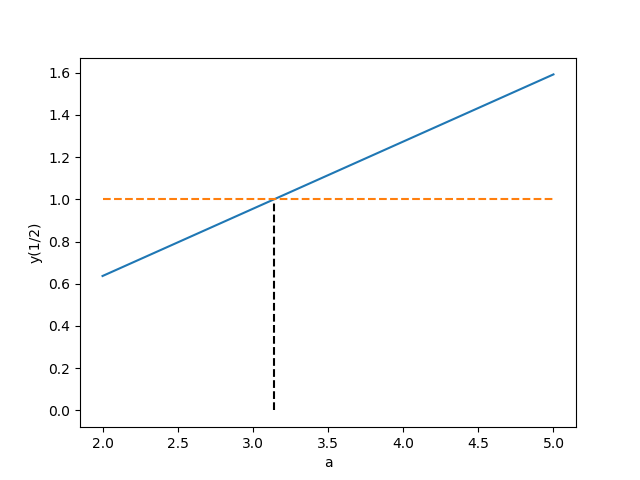
\includegraphics[scale=0.750]{4.png}\\
The actual plot of $\sin(x)$ is plotted below alongside the two closest approximations we obtained using the shooting method\\
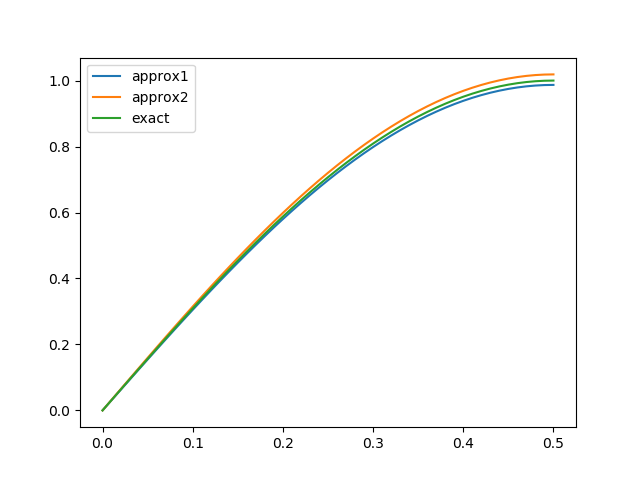
\includegraphics[scale=0.75]{4_Shooting_function_Plot.png}\\
It can be seen that the obtained functions closely approximate $sin(x)$, any deviation from the actual function can be attributed to a large stepsize of $0.1$ for the $a$ value.
	
\end{document}